\section{Arquitetura do Sistema}

    Na interseção descrita na figura \ref{fig:diagramaEstrada} existem 4 semáforos, pelo que, idealmente, cada um seria representado por uma raspberrypi. Contudo, devido ao facto de apenas existirem duas raspberrypis disponíveis, os semáforos 1 e 3 são representados pela mesma raspberrypi e os semáforos 2 e 4 por outra, sendo que é considerado que quando os semáforos 1 e 3 têm sempre o mesmo e os semáforos 2 e 4 também. Assim, quando a raspberrypi A está no estado VERDE é permitido o transito horizontal e quando a raspberrypi B está VERDE é permitido o trânsito vertical. As raspberrypis nunca apresentam o mesmo estado em simultâneo. 

    O sistema foi desenhado de acordo com a figura \ref{fig:diagramaSistema}. Ambas as raspberrypis foram conectadas à rede Wi-Fi do portátil que por sua vez comunica com o servidor NTP \url{pool.ntp.org}. As cada raspberrypi representa um cliente que envia para o portátil os pedidos NTP de acordo com a secção \ref{sec:NTP} que por sua vez são reencaminhados para o servidor. A resposta faz o caminho oposto.
    O estado da cada raspberrypi é enviado para o portátil cada vez que existe uma transição. Este processo serve apenas para monitorização e está representado na figura como monitor. Este regista o tempo local de chegada da mudança de estado de cada estado e avalia a diferença de tempo entre a chegada do estado de cada raspberrypi. Por exemplo, quando A fica VERMELHO B deve ficar VERDE, o monitor avalia o desfasamento desta duas ações (que deve ser o menor possível).

    O protocolo empregue para a comunicação é o "Transmission Control Protocol" - TCP. Se o servidor NTP não responder à solicitação, é acionado um "timeout", e o sistema tenta restabelecer a ligação. Esta funcionalidade é crucial, uma vez que o servidor tem uma disponibilidade muito baixa, mas um tempo médio de reparação reduzido, permitindo assim uma rápida recuperação da ligação. Isso resulta em correções não periódicas, mas essa irregularidade não afeta significativamente a sincronização do sistema já que o sistema esforça-se para restabelecer a ligação o mais rapidamente possível. Para além disso, o facto do servidor responder em $t$ ou $t + 1$ não tem grande influência no ajuste, já que os relógios das raspberrypis continua a utilizar parâmetros antigos para a correção e não é esperado que estes se alterem subitamente.


    \begin{figure}[h]
        \centering
        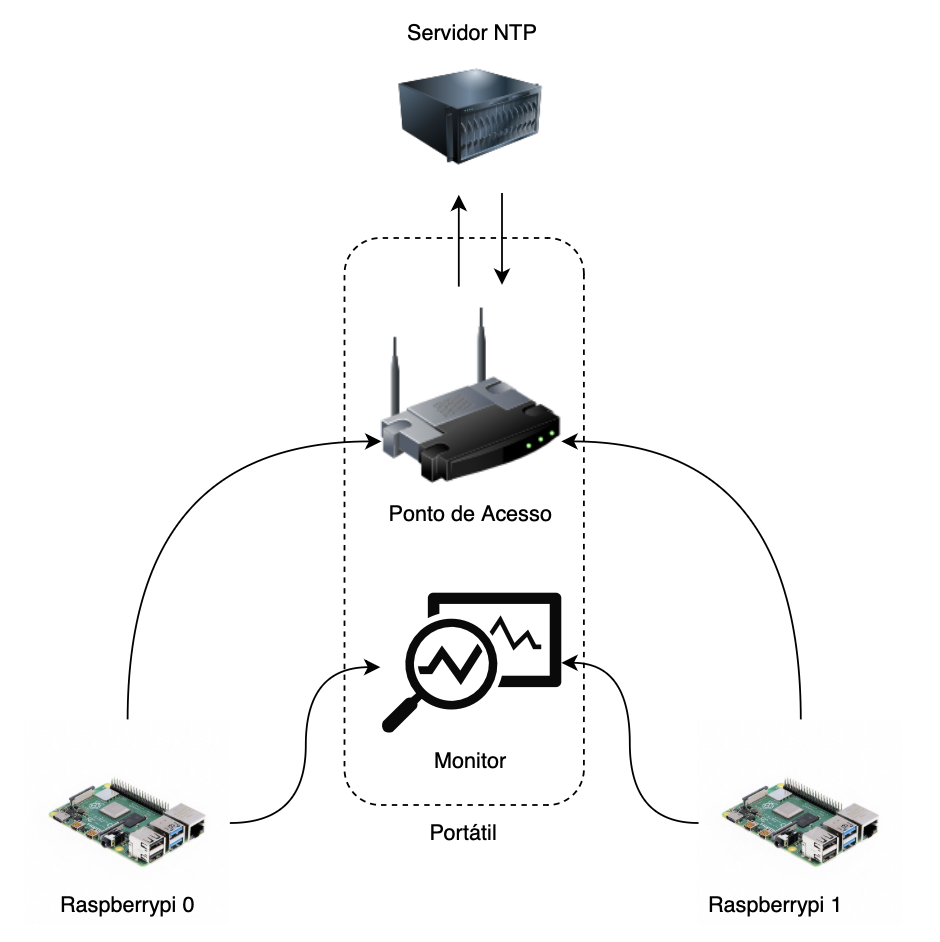
\includegraphics[width=0.8\linewidth]{figures/diagramaSistema.png}
        \caption{Diagrama da arquitetura do sistema \cite{b1}}
        \label{fig:diagramaSistema}
    \end{figure}


    